\PassOptionsToPackage{unicode=true}{hyperref} % options for packages loaded elsewhere
\PassOptionsToPackage{hyphens}{url}
\PassOptionsToPackage{dvipsnames,svgnames*,x11names*}{xcolor}
%
\documentclass[a4paper]{article}
\usepackage{lmodern}
\usepackage{amssymb,amsmath}
\usepackage{ifxetex,ifluatex}
\usepackage{fixltx2e} % provides \textsubscript
\ifnum 0\ifxetex 1\fi\ifluatex 1\fi=0 % if pdftex
  \usepackage[T1]{fontenc}
  \usepackage[utf8]{inputenc}
  \usepackage{textcomp} % provides euro and other symbols
\else % if luatex or xelatex
  \usepackage{unicode-math}
  \defaultfontfeatures{Ligatures=TeX,Scale=MatchLowercase}
\fi
% use upquote if available, for straight quotes in verbatim environments
\IfFileExists{upquote.sty}{\usepackage{upquote}}{}
% use microtype if available
\IfFileExists{microtype.sty}{%
\usepackage[]{microtype}
\UseMicrotypeSet[protrusion]{basicmath} % disable protrusion for tt fonts
}{}
\IfFileExists{parskip.sty}{%
\usepackage{parskip}
}{% else
\setlength{\parindent}{0pt}
\setlength{\parskip}{6pt plus 2pt minus 1pt}
}
\usepackage{xcolor}
\usepackage{hyperref}
\hypersetup{
            pdftitle={Dashboard Manual Part 2},
            pdfauthor={Michael Wild},
            colorlinks=true,
            linkcolor=Maroon,
            filecolor=Maroon,
            citecolor=Blue,
            urlcolor=blue,
            breaklinks=true}
\urlstyle{same}  % don't use monospace font for urls
\usepackage{longtable,booktabs}
% Fix footnotes in tables (requires footnote package)
\IfFileExists{footnote.sty}{\usepackage{footnote}\makesavenoteenv{longtable}}{}
\usepackage{graphicx,grffile}
\makeatletter
\def\maxwidth{\ifdim\Gin@nat@width>\linewidth\linewidth\else\Gin@nat@width\fi}
\def\maxheight{\ifdim\Gin@nat@height>\textheight\textheight\else\Gin@nat@height\fi}
\makeatother
% Scale images if necessary, so that they will not overflow the page
% margins by default, and it is still possible to overwrite the defaults
% using explicit options in \includegraphics[width, height, ...]{}
\setkeys{Gin}{width=\maxwidth,height=\maxheight,keepaspectratio}
\setlength{\emergencystretch}{3em}  % prevent overfull lines
\providecommand{\tightlist}{%
  \setlength{\itemsep}{0pt}\setlength{\parskip}{0pt}}
\setcounter{secnumdepth}{5}
% Redefines (sub)paragraphs to behave more like sections
\ifx\paragraph\undefined\else
\let\oldparagraph\paragraph
\renewcommand{\paragraph}[1]{\oldparagraph{#1}\mbox{}}
\fi
\ifx\subparagraph\undefined\else
\let\oldsubparagraph\subparagraph
\renewcommand{\subparagraph}[1]{\oldsubparagraph{#1}\mbox{}}
\fi

% set default figure placement to htbp
\makeatletter
\def\fps@figure{htbp}
\makeatother

\usepackage{fancyhdr}
\pagestyle{fancy}
\chead{
\includegraphics[width=3cm, height=1cm]{logo_wb_data.jpg}}
\usepackage{tcolorbox}
\usepackage{titling}
\pretitle{\begin{center} 
\includegraphics[width=2in,height=2in]{logo_suso.png}\LARGE\\}
\posttitle{\end{center}}

\title{Dashboard Manual Part 2}
\author{Michael Wild}
\date{3/12/2020}

\begin{document}
\maketitle

{
\hypersetup{linkcolor=}
\setcounter{tocdepth}{2}
\tableofcontents
}
\newpage

\hypertarget{background}{%
\section{Background}\label{background}}

This is the second part of the 2-part manuals accompanying the census dashboard. It is intended to be read by the census quality control team (i.e.~supervisors/headquarters) as it will describe the full \textbf{monitoring} process.

The first part of the manuals deals with the set-up of the application, and is only intended for the main census (IT) manager. None of these functions are intended to be used by the common user of this application.

In the following we will describe the workflow, as it was understood by our team, as well as the different functions in the application, covering this workflow. Since the application uses the Survey Solutions API (Application Programming Interface, used to connect third party Software to Survey Solutions), and is fully integrated with Survey Solutions through this API, we will also stick to the Survey Solutions terminology. This means:

\begin{itemize}
\tightlist
\item
  \textit{Headquarters} refers to Survey Solutions Headquarters
\item
  \textit{Supervisors} refers to Survey Solutions Supervisors
\item
  \textit{Interviews, Assignments etc.} as well.
\end{itemize}

Besides starting the automation, the application is build to facilitate the quality control for large scale listing operations including the collection of geo-referenced location data for each census unit. The application is build around the Survey Solutions Computer Assisted Survey System (CASS) and its API. It is written in the open source programming language R and uses the R shiny package for building the graphical user interface (GUI). \newline

It also uses the recently released \texttt{SurveySolutionsAPI} package (\url{https://github.com/michael-cw/SurveySolutionsAPI}) to communicate with the Survey Solutions CASS.

\newpage

\hypertarget{operations}{%
\section{Operations}\label{operations}}

The workflow as understood by the Survey Solutions Team formed the basis for this application. It is intended to be used by the \underline{central quality control team} which should consist of 5 to 10 persons. Since some of the processes conducted by the application require large scale data operations, there should never be more than 5 simultaneous users, as otherwise the processes may slow down significantly. In addition this application should also only be used by persons who received training and have studied this manual.

Main features of the operation are:

\begin{itemize}
\tightlist
\item
  continuous monitoring of the listing progress
\item
  continuous monitoring of the listing data
\item
  generation of reports for field teams
\item
  automated procedures for quality control
\item
  manual procedures of for quality control
\item
  generation of base maps (requires ESRI license to access the \url{https://tiledbasemaps.arcgis.com/arcgis/ World Imagery data})
\item
  \textbf{census} or \textbf{sample mode}.
\end{itemize}

\begin{tcolorbox}[colback=red!5,colframe=red!40!black,title=Important]
It is important to note, that the monitoring version of this application has 2 very important characteristics.
\begin{enumerate}
    \item This application is independent of the Survey Solutions server. Besides resetting an assignment (as described in Section 2.5, Control set 3), non of the actions undertaken in this application has any permanent effect on the data stored on the server.
    \item The automation is independent of the application. This means non of the actions you undertake here, even crashing the application would anyhow affect the automation process. This process can only be stopped through the version used by the main census (IT) manager.
\end{enumerate}
\end{tcolorbox}
\newpage

The underlying work process has been understood as depicted in the following process diagram:

\begin{figure}

{\centering 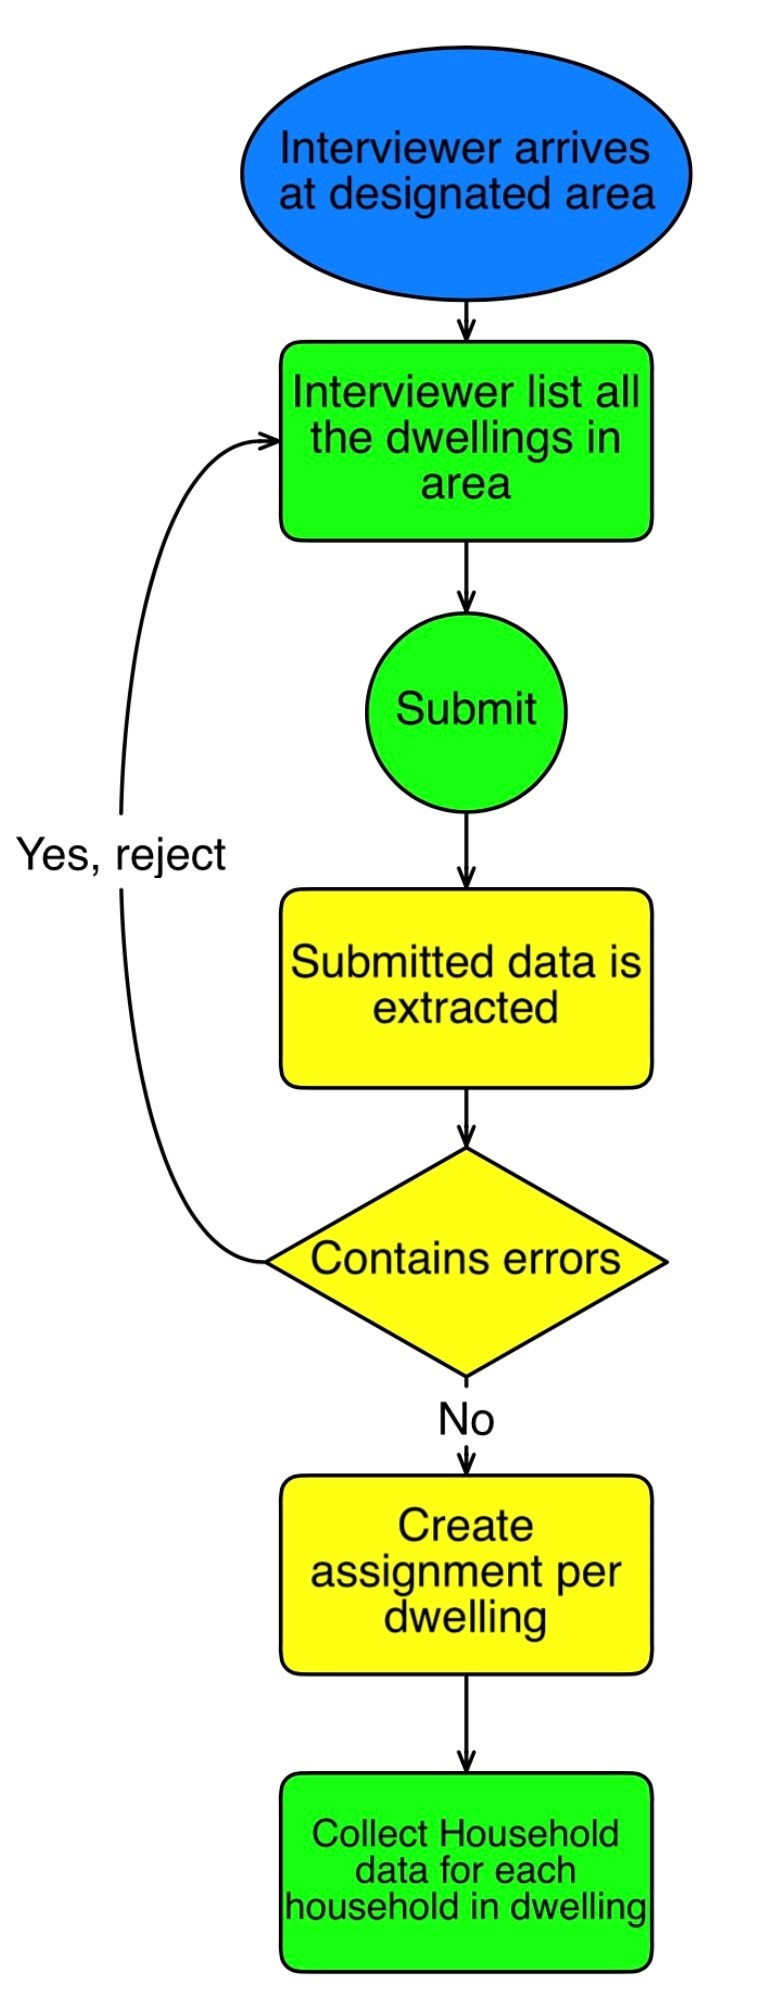
\includegraphics[width=1.28in]{proc1flow} 

}

\caption{Workflow Listing}\label{fig:proc1}
\end{figure}

The main assumption behind (Figure \ref{fig:proc1}) for the provided version of this dashboard is that there is a \underline{single interviewer for each enumeration area}. After successfully completing the listing, the interviewer submits the interview containing the enlisted structures/dwellings to the server. If this happens without error, the interviewer will receive - \underline{through a second synchronization} - in return, a set of new assignments for each of the private, non-abandoned dwelling. These new assignments also include the exact geo-referenced location for the structure in which the dwelling for the main enumeration is located. With this location information, the interviewer can subsequently navigate to the structure (i.e.~by using Google maps, maps.me or any other navigation application), and conduct the enumeration (main interview) for each of the dwellings.

\newpage

\hypertarget{login}{%
\subsection{Login}\label{login}}

To login to the application please use \textbf{ONLY} the following link: \url{https://apps4dev.mysurvey.solutions/SuSo_Bahamas2020/}. The credentials for the login have been provided through an email to the census management.

\begin{figure}

{\centering 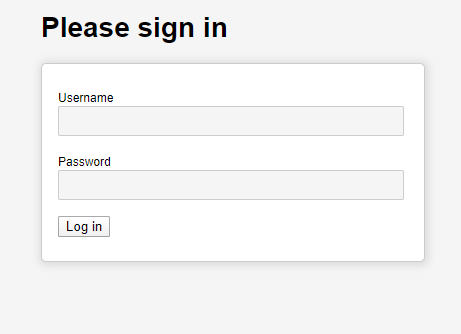
\includegraphics[width=1.15in]{login} 

}

\caption{Application Login}\label{fig:login}
\end{figure}

\newpage

\hypertarget{assignment-automation}{%
\subsection{Assignment Automation}\label{assignment-automation}}

After logging in, you will see the first Section ``Assignment Automation''. In this section, there are no controls available for this version of the application. Users logged in, can however monitor the process through the center box.

\begin{figure}

{\centering 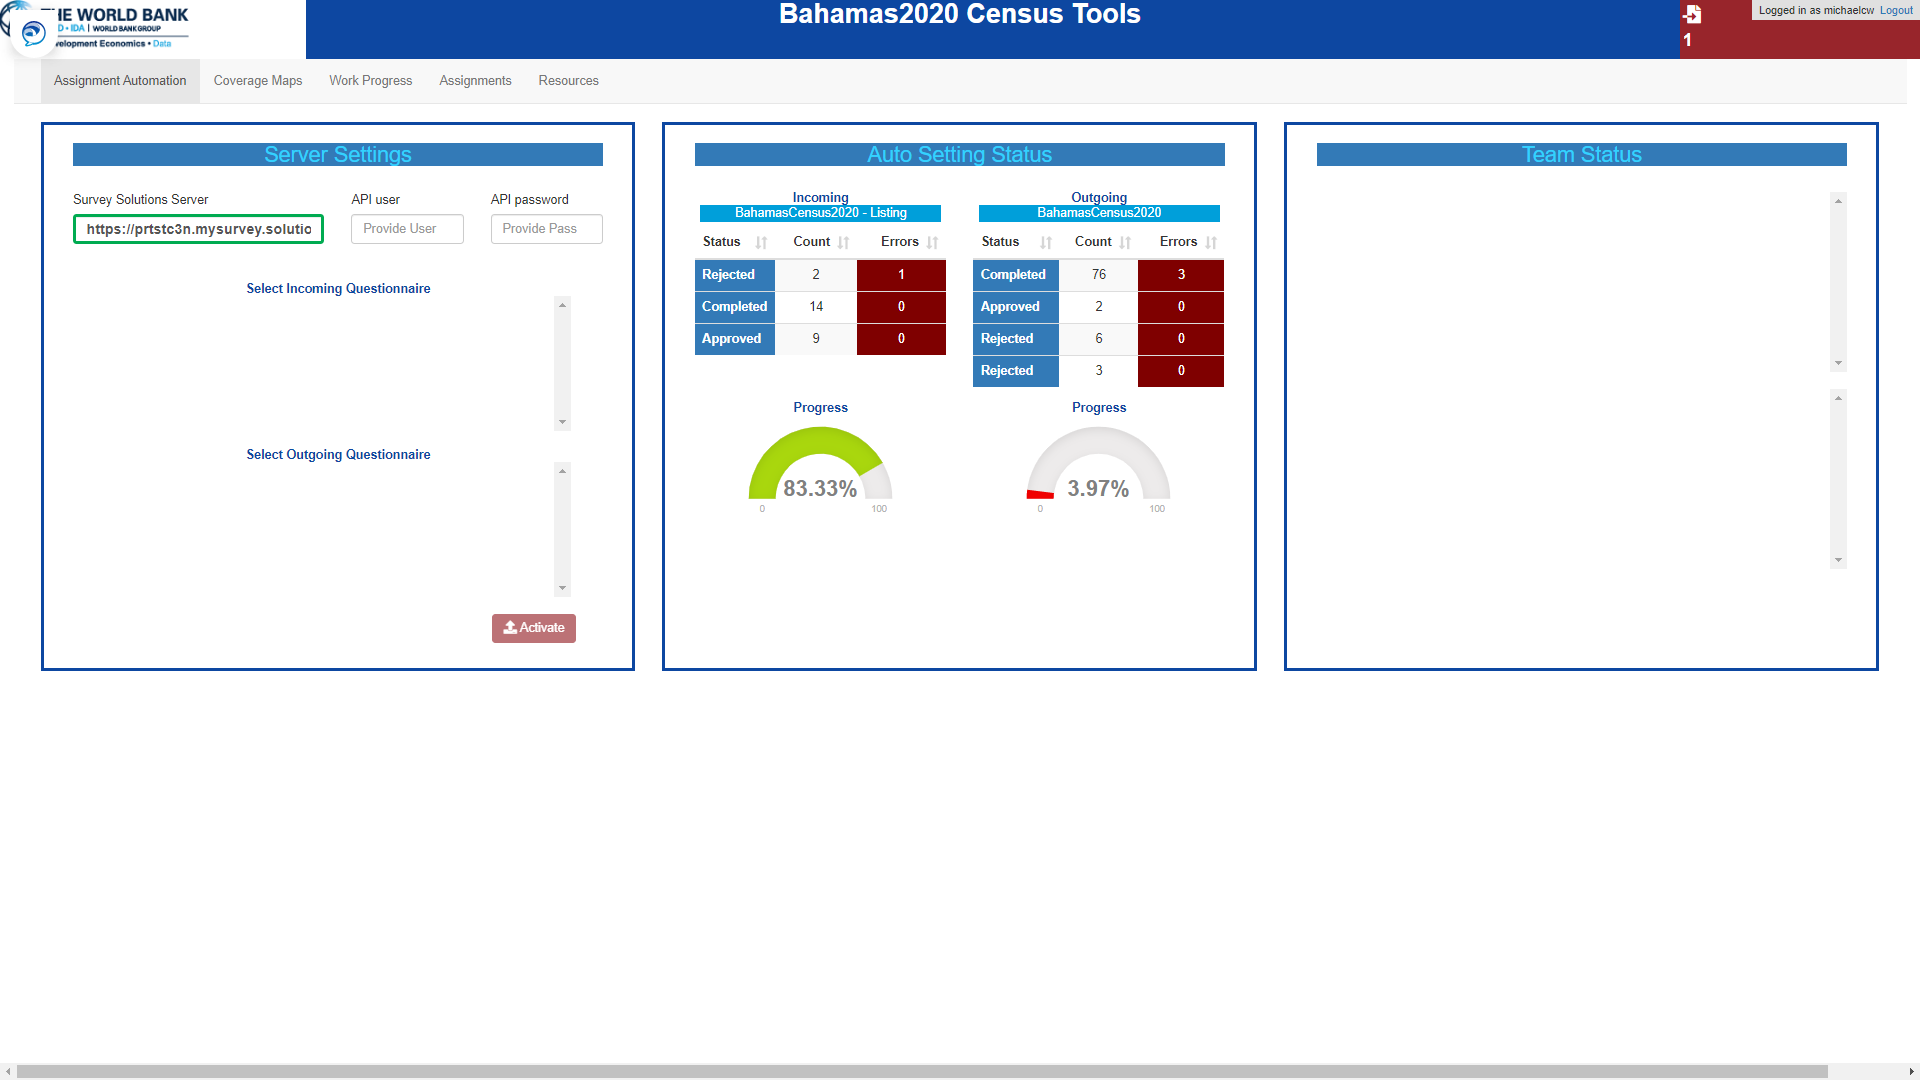
\includegraphics[width=4.8in]{tab1} 

}

\caption{Assignment Automation}\label{fig:tab1}
\end{figure}

The left table and gauge in the center box shows the progress of the incoming (listing) data collection, the right table and gauge the progress for the outgoing (enumeration) questionnaire. This is it for this page, no other options are available to the monitoring user.

\newpage

\hypertarget{coverage-maps}{%
\subsection{Coverage Maps}\label{coverage-maps}}

The coverage maps display the overall progress of the incoming data by location. All submitted interviews will be displayed here according to the collected geo-locations. In addition, the map also displays the provided boundary files. Main features of this section are:

\begin{itemize}
\tightlist
\item
  The map updates with any submission
\item
  The map displays processed and rejected interviews
\item
  The map displays the data by building type.
\end{itemize}

\begin{figure}

{\centering 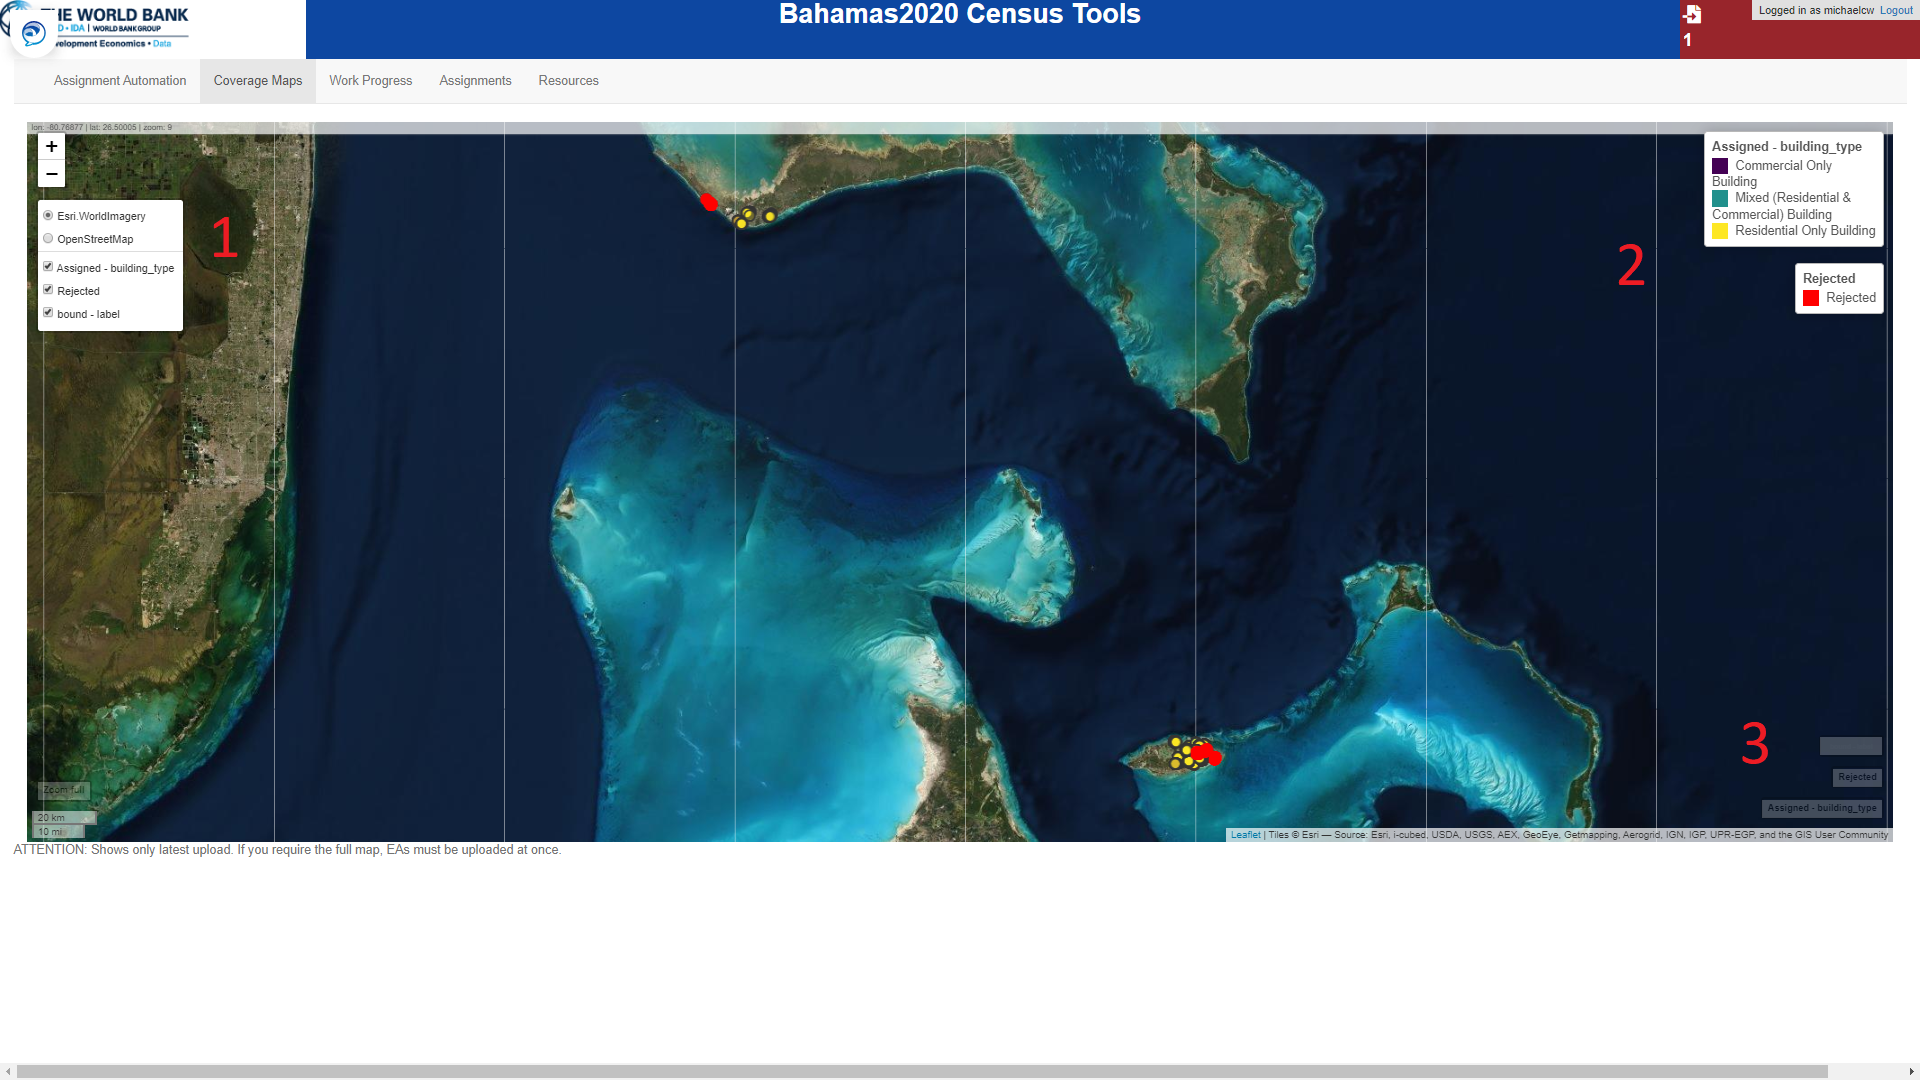
\includegraphics[width=4.8in]{tab2} 

}

\caption{Coverage Maps}\label{fig:tab2}
\end{figure}

\textcolor{red}{Control set 1} allows for the selection of the underlying base map (satellite/open street map), as well as the different types of incoming data. These are:

\begin{itemize}
\tightlist
\item
  Processed Incoming
\item
  Rejected Incoming
\item
  Enumeration area boundaries.
\end{itemize}

These can be selected/unselected as required. \newline

\textcolor{red}{Control set 2} is the legend for all the different colors used in the map. The different colors reflect the building types. \newline

\textcolor{red}{Control set 3} allows the user to quickly zoom to the corresponding data set. Clicking on it will center the map on the requested data.
\newpage

\hypertarget{work-progress}{%
\subsection{Work Progress}\label{work-progress}}

The Work Progress section allows you to

\begin{itemize}
\tightlist
\item
  monitor the responses to the different questions in the \underline{incoming questionnaire}, check if expected and real distribution of
\item
  generate reports for teams, overall and for paradata (i.e.~how many seconds per question), which can be used by quality control team
\item
  review collection for individual enumeration areas.
\end{itemize}

\begin{figure}

{\centering 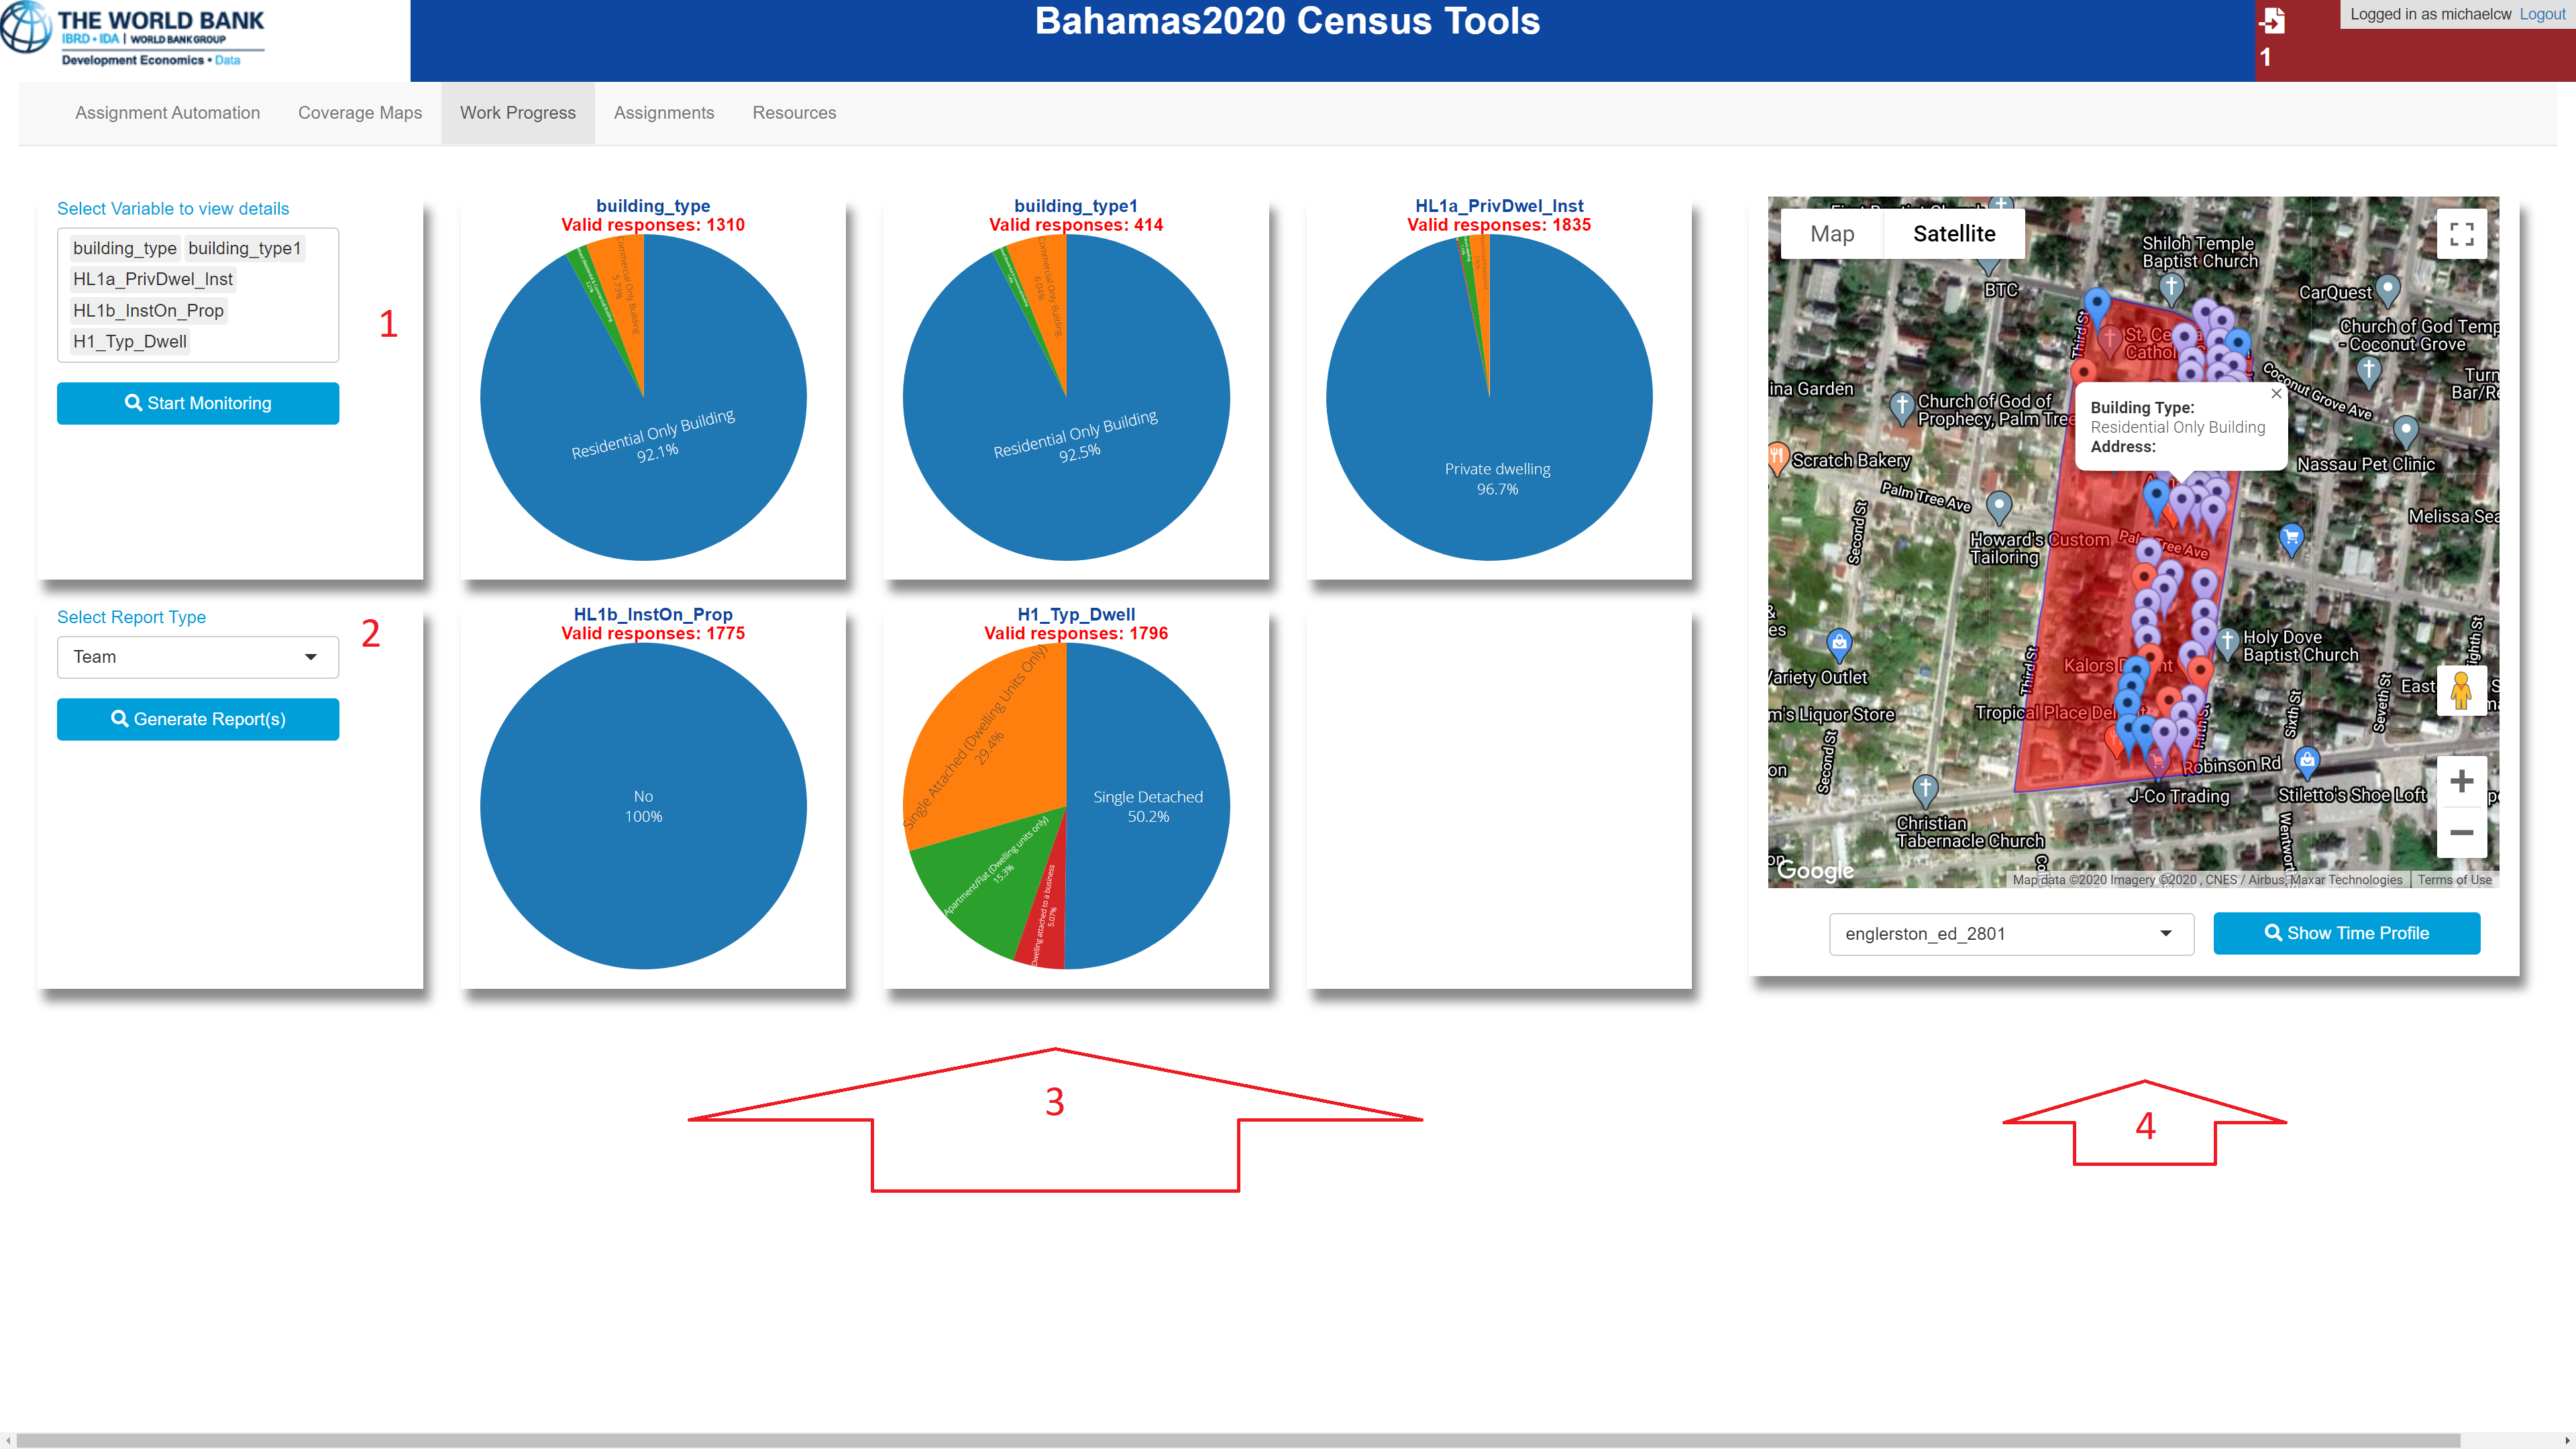
\includegraphics[width=4.8in]{tab3} 

}

\caption{Work Progress}\label{fig:tab3}
\end{figure}

\textcolor{red}{Control set 1} allows you to select the variables which you want to monitor. Up to 6 variables can be observed simultaneously, and you can always modify the selection. After your selection in the upper box, confirm your selection by clicking the lower light-blue button. If valid responses had been submitted, you will see their distribution here. Only categorical question types are reported.\newline
\textcolor{red}{Control set 2} is for the generation of reports. Currently the application generates an overall report for each of the incoming data items, a similar report by supervisor and a paradata report (select this option carefully since processing may take longer.) \newline
\textcolor{red}{Control set 3} is the plot section. Up to 6 plots can be generated simultaneously. The values displayed refer to their percentage shares in the total number of \underline{valid responses}.\newline
\textcolor{red}{Control set 4} is the single shape viewer. Select an ED from the drop down menu, to view only this area and its data if available. The map allows to view the Google satellite image through the selection panel in the upper left corner. In the upper right corner it is also possible to extend the map to the full screen. Different colors refer to different building types. The \textcolor{cyan}{light blue button} also allows you to review the timeline for this questionnaire in the selected area, as a process model (see for details: \url{https://www.bupar.net/}). Generation of this may take a bit of time. After clicking the button a pop-up window will appear as described in the next section.

\hypertarget{survey-process-data-paradata}{%
\subsubsection{Survey Process Data (= Paradata)}\label{survey-process-data-paradata}}

At the same time as the pop up up window appears a loading screen shows up in the upper right corner. Wait until this process is finished, and then the graph will be displayed.
Currently the available paradata graphs are the complete timeline of the data collection process in seconds. This displays for example, the pace of the data collection process in this area in seconds and for each question.

The other available paradata graph displays a summary of all the interviewer actions on the device during \underline{the whole data collection process}. It displays for example how many answers and how many times answers had been removed, or how many times the data collection process had been paused.

\begin{figure}
    \centering
    \begin{minipage}{0.48\textwidth}
        \centering
        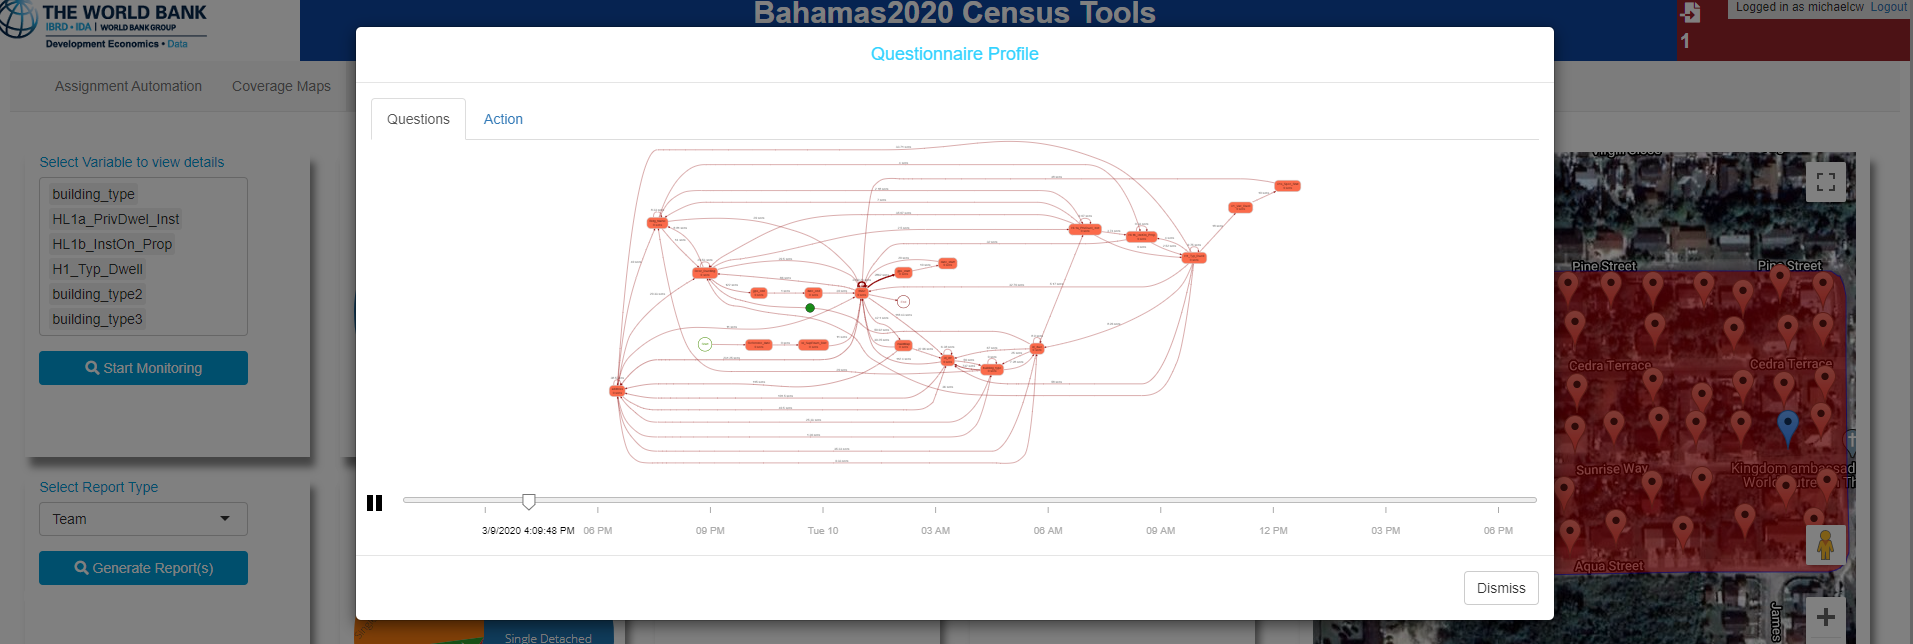
\includegraphics[width=1\textwidth]{modal_questions.png} % Timeline by question
        \caption{Timeline by question}
    \end{minipage}\hfill
    \begin{minipage}{0.48\textwidth}
        \centering
        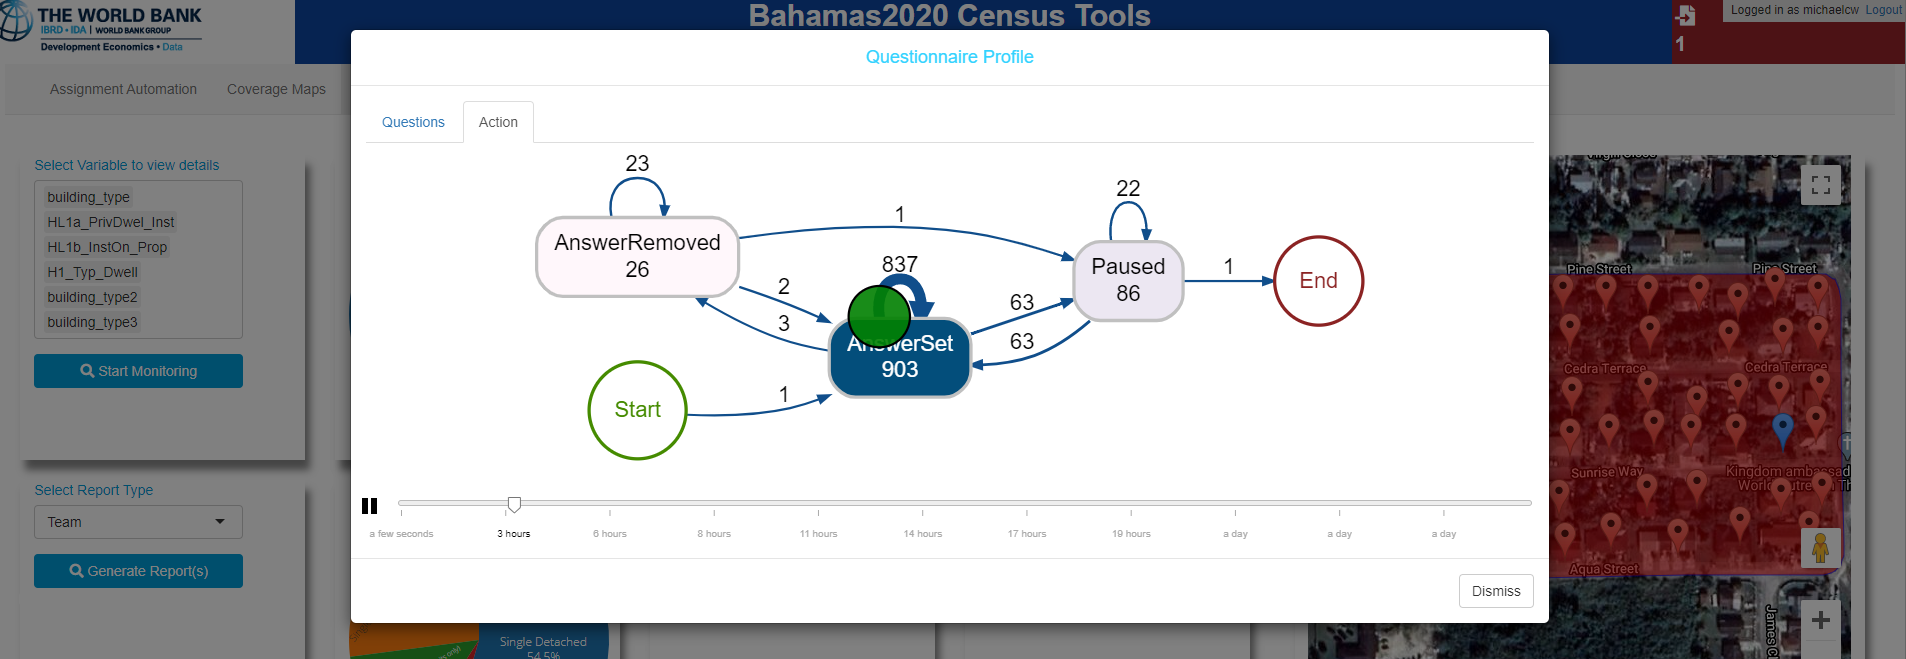
\includegraphics[width=1\textwidth]{modal_actions.png} % Summary of actions
        \caption{Summary of actions}
    \end{minipage}
\end{figure}
\newpage

\hypertarget{assignments}{%
\subsection{Assignments}\label{assignments}}

The Assignments section allows you to monitor the data flow at the level of the individual assignment, in particular it allows you to:

\begin{itemize}
\tightlist
\item
  see the number of rejections by interview, and inspect rejected questionnaires in Survey Solutions
\item
  see the assignments created for each of the correctly submitted incoming interviews
\item
  reset the incoming interview to its unsubmitted states.
\end{itemize}

\begin{figure}

{\centering 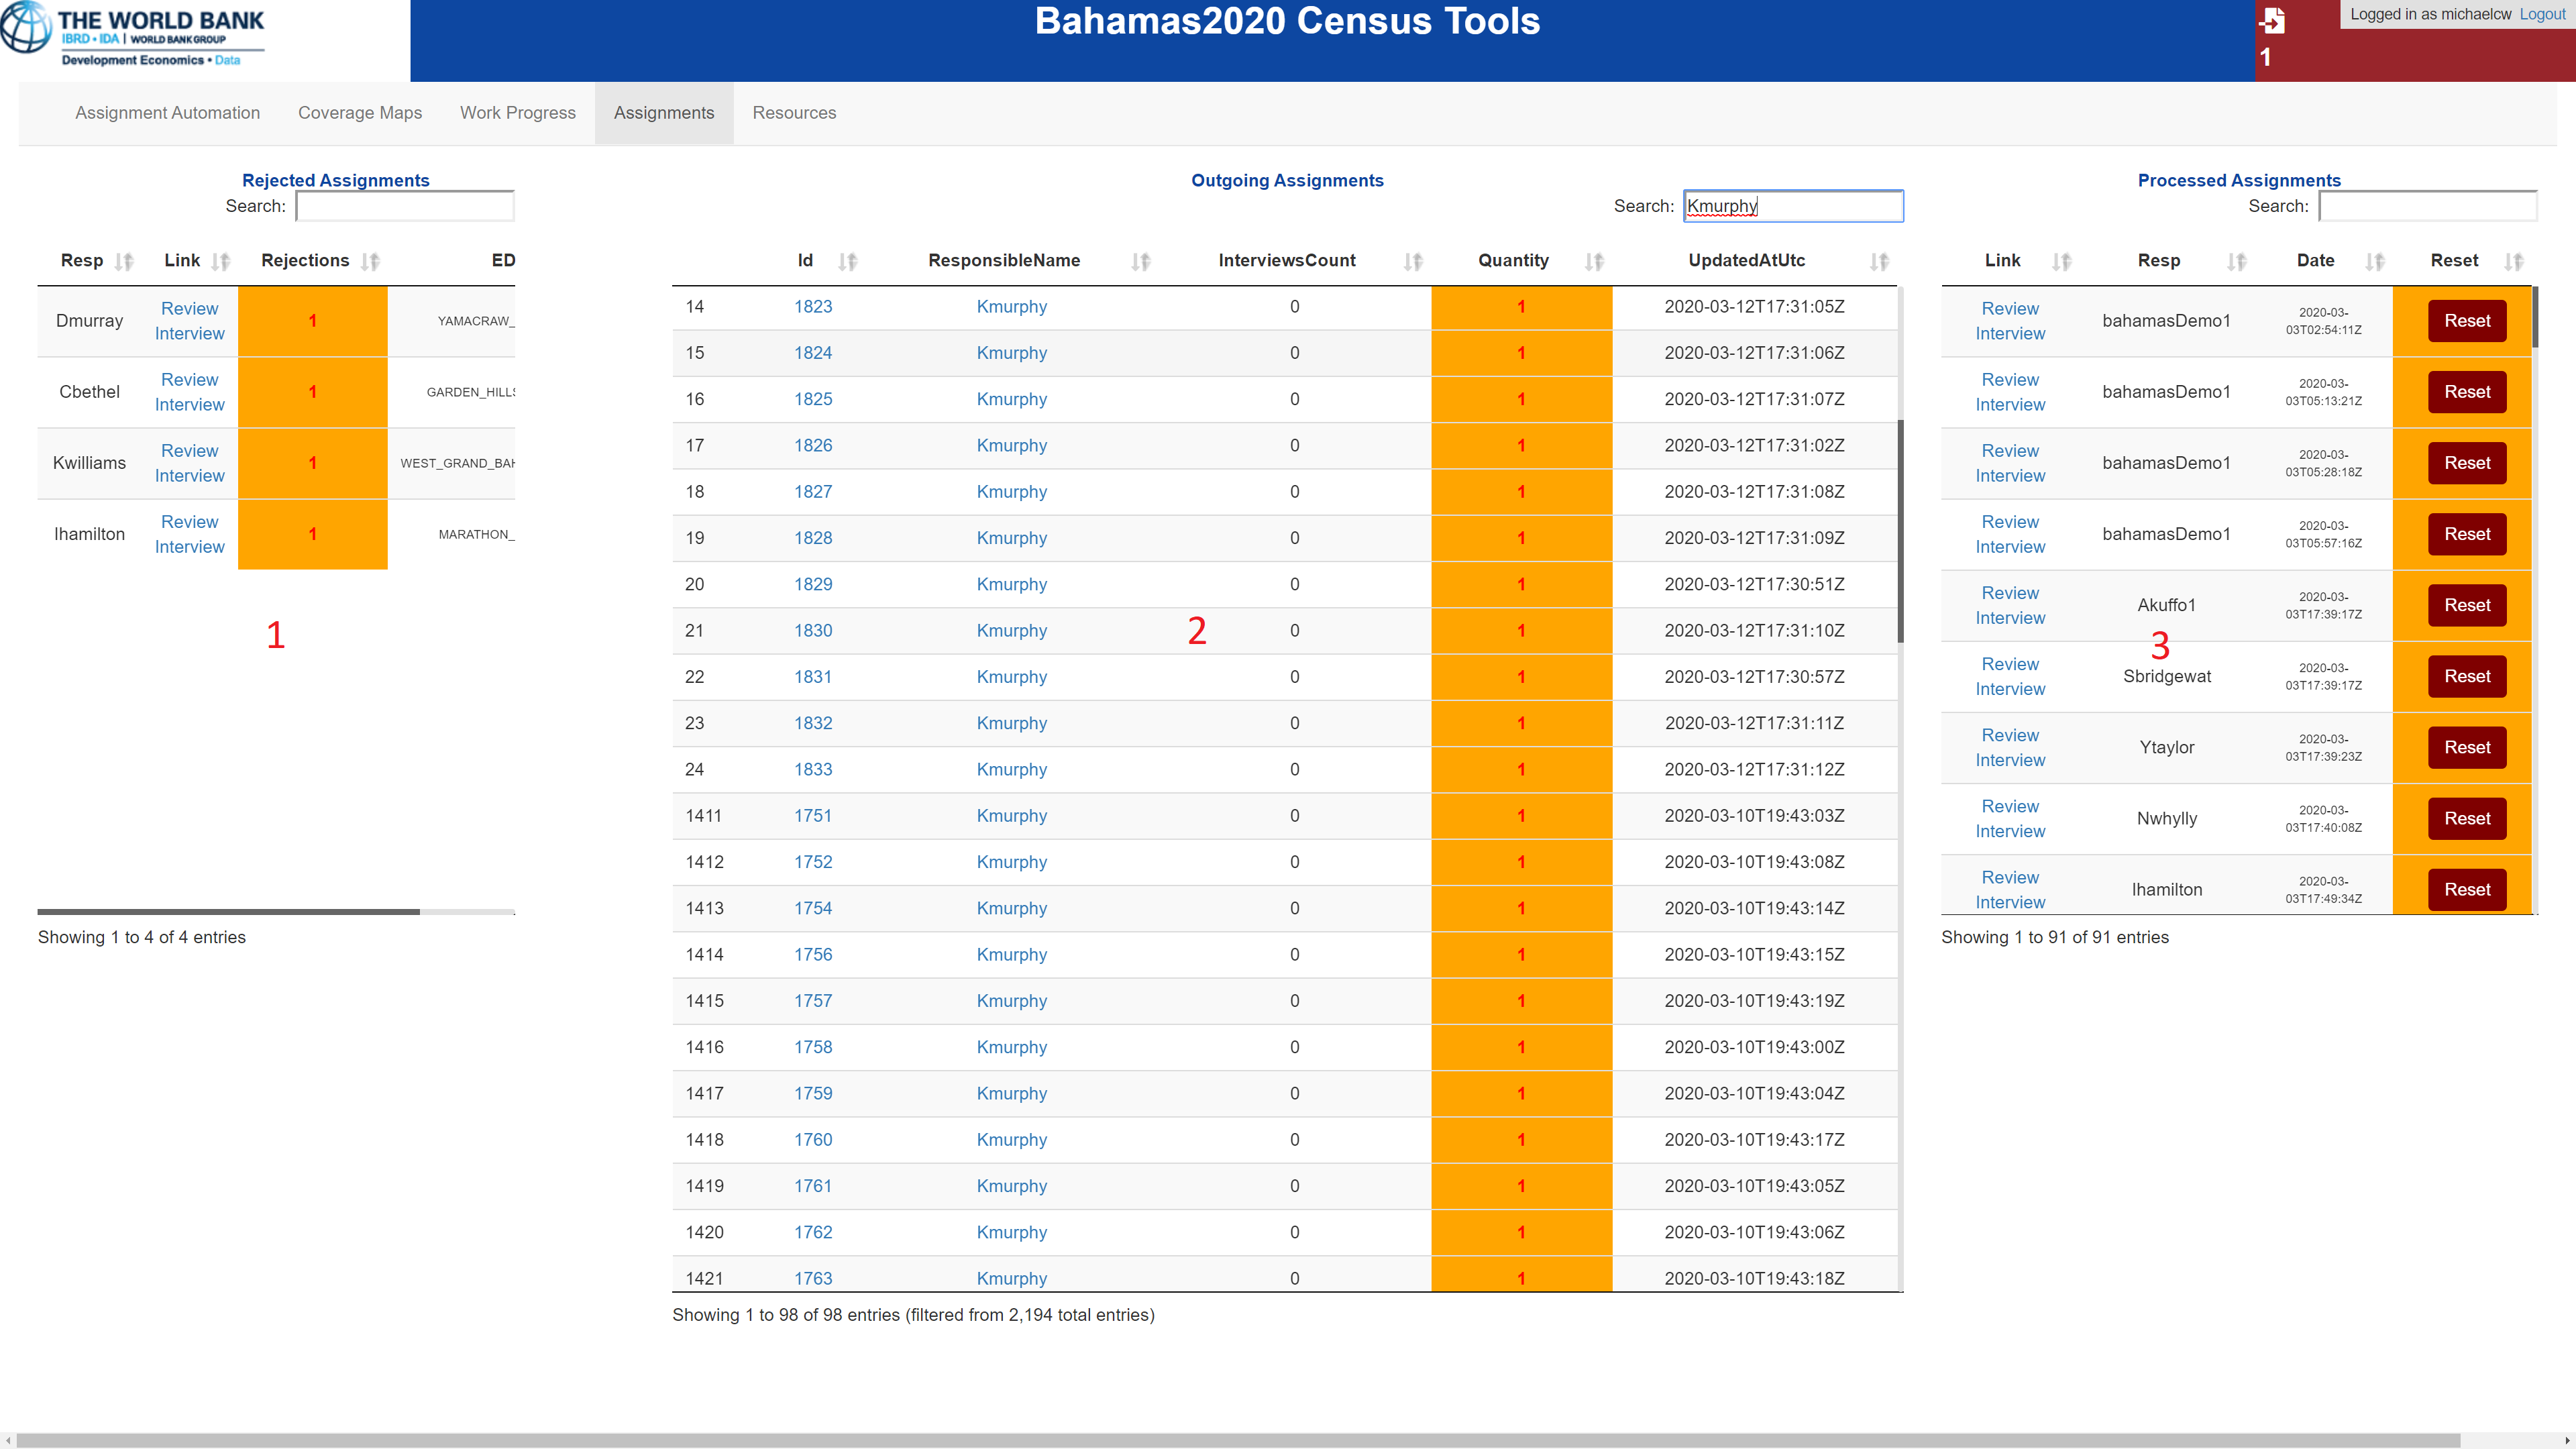
\includegraphics[width=4.8in]{tab4} 

}

\caption{Assignments}\label{fig:tab4}
\end{figure}

\textcolor{red}{Control set 1} provides information on all the interviews rejected in the current survey. Clicking on the link the corresponding column for a specific interview will open a new browser window, and open the underlying questionnaire \underline{one your Survey Solutions server}. For this purpose \underline{the user has to be logged in to the Survey Solutions server}, and also have the permission to view this data (i.e.~headquarters, or supervisors for team members. This functionality could also be used to reassign the interview, i.e.~if a certain interviewer produces to many rejections. \newline
\textcolor{red}{Control set 2} shows all the created outgoing assignments as well as their status. It also contains a link to the corresponding assignment details (Id), or to the corresponding responsible interviewer (ResponsibleName). \newline
\textcolor{red}{Control set 3} \textcolor{blue}{ATTENTION: ACTIONS IN THIS TABLE ARE IRREVERSIBLE. RESETTING AN INTERVIEW DELETES ALL CREATED ASSIGNMENTS INCLUDING THEIR DATA. USE ONLY AFTER CAREFUL PREPARATION!!.} In this table you an see all the processed incoming interviews. In the column Link, you can open the interview directly on the Survey Solutions server. In cases were it is necessary to send the listing questionnaire back to the interviewer, or to take the questionnaire out of the automation process, you can reset the interview to its state before synchronization. As a result the questionnaire is rejected to the user, including the data before submission, the interview id is taken out of the submission data base (=the interviewer can resubmit), and the created assignments are deleted (\textbf{Attention: Assignments are also deleted, if they contain data, so prepare carefully!}). After clicking the red button, an additional popup window will show up, which requires you to confirm the operation, by re-entering the displayed questionnaire Id. \newline

\begin{figure}
    \centering
    \begin{minipage}{0.48\textwidth}
        \centering
        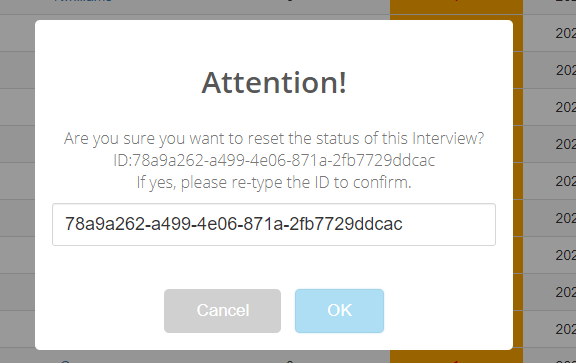
\includegraphics[width=1\textwidth]{modal_reset.png} % Timeline by question
        \caption{first figure}
    \end{minipage}\hfill
    \begin{minipage}{0.48\textwidth}
        Figure 9 shows the confirmation dialogue. After confirming with OK, the process will be started, and can not be reversed.
    \end{minipage}
\end{figure}
\newpage
\newpage

\hypertarget{resources}{%
\subsection{Resources}\label{resources}}

In this section you can:

\begin{itemize}
\tightlist
\item
  change the boundaries visible in the Coverage Map
\item
  create the TPK (map package) as well as its corresponding boundary file for the Survey Solutions interviewer application.
\item
  download and delete the current log file for the automation process (a new one will be create as soon as the process is executed again).
\end{itemize}

\begin{figure}

{\centering 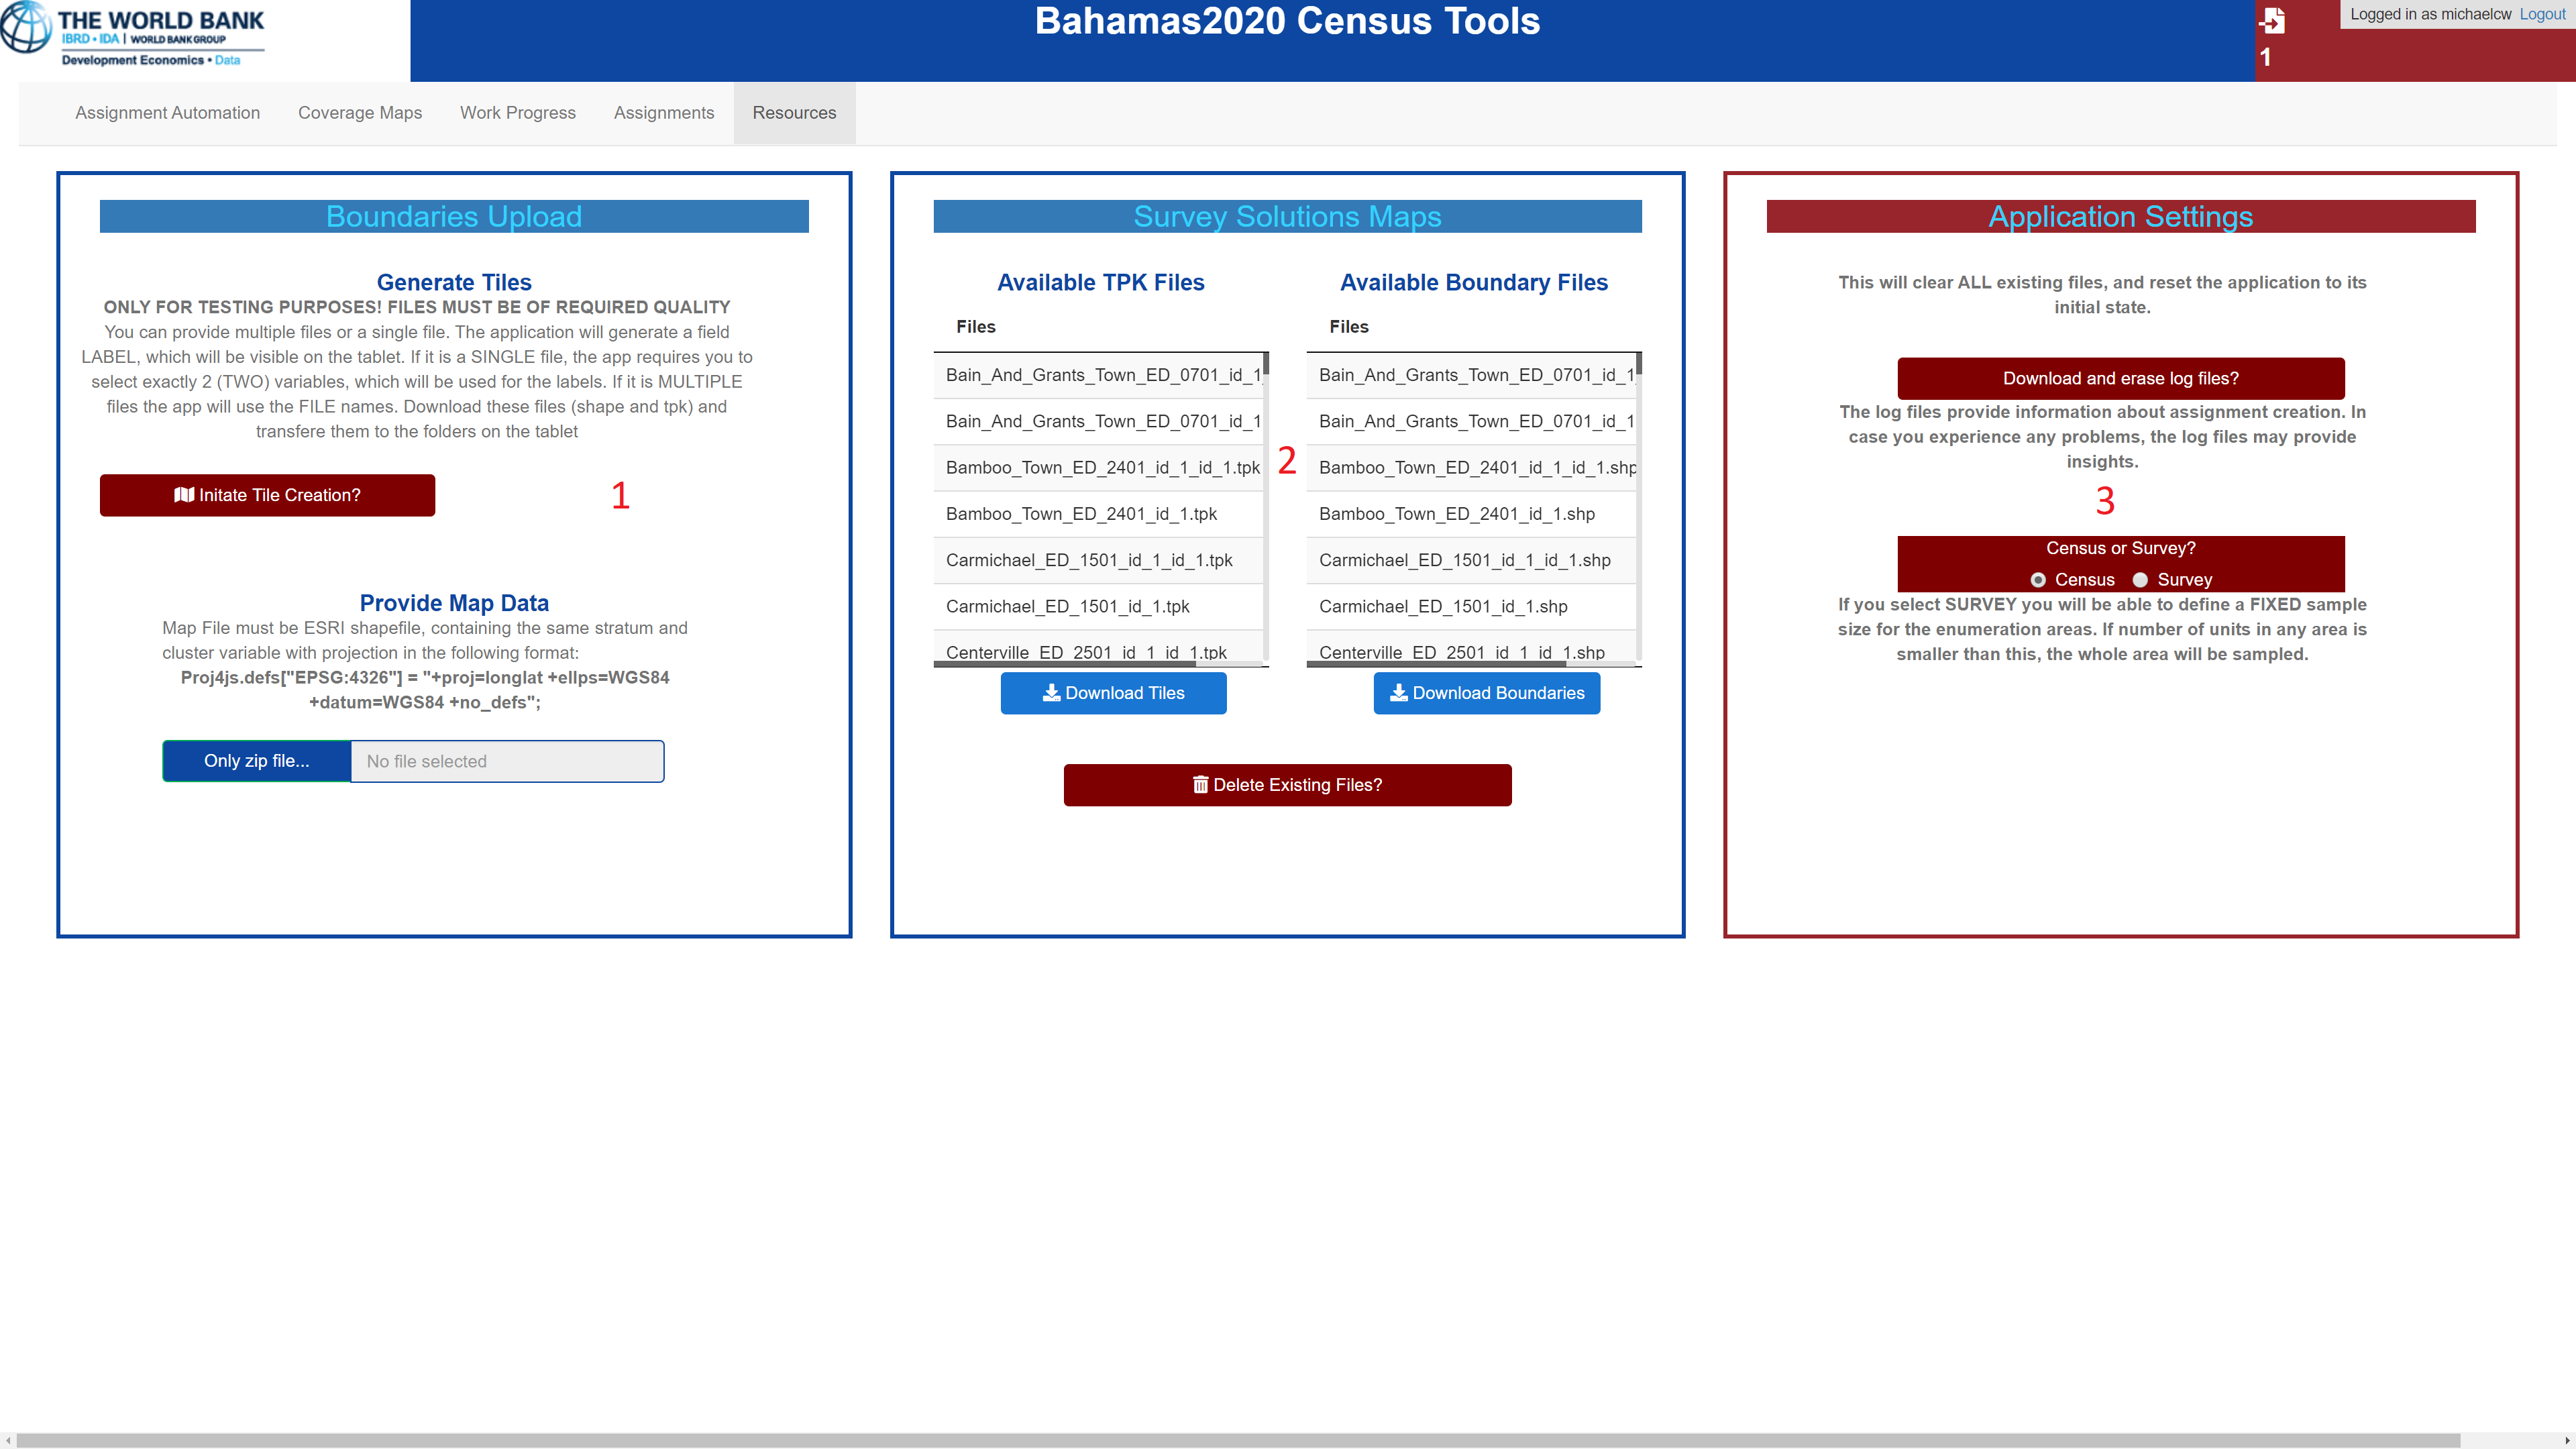
\includegraphics[width=4.8in]{tab5} 

}

\caption{Resources}\label{fig:tab5}
\end{figure}

\textcolor{red}{Control set 1} allows you to upload the map file(s). It allows for the upload of a SINGLE boundary file or MULTIPLE boundaries. To successfully use the uploaded geo-spatial data, it needs to meet certain minimum requirements.

\begin{tcolorbox}[colback=cyan!5,colframe=cyan!40!black,title=Requirements for area boundaries:]
\begin{enumerate}
    \item Contain the minimum components for a shape file including its projection.
    \item Must include the required naming convention (i.e. have a unique Id) for each segment.
    \item The file(s) must be packed in a zip-file at the FIRST folder level\footnote{This means the zip-file should not contain a folder containing all the files, but instead contain the files themselves. To achieve this, you need to select the files themselves (NOT their folder), when creating the zip-archive.}.
\end{enumerate}
\end{tcolorbox}

After uploading the files, the old map files in the coverage map are replaced by the new files. You can replace files anytime. If you choose to produce the TPK files, click the corresponding red button. When the process is finished, the files will be visible in Control set 2.
\newline
\textcolor{red}{Control set 2} allows you to download the files. It is recommended, to use both files for the data collection process. Clearing the directory is also possible. This will delete all the files, it will however not delete the currently visible Coverage Map. The boundaries in this map are replaced with EACH upload.\newline
\textcolor{red}{Control set 3} finally has only one available functionality, which is to download the automation log-file. In the log file, you can find information about the automation process, and in particular about failure and success. \underline{Only use this after instructed to do so}. \newline

\end{document}
